\documentclass[../../masterdoc]{subfiles}
% Hier m�ssen keine Packages geladen werden, es werden automatisch die von masterdoc geladen,
% sowie die Konfigurationen.
\begin{document}

\chapter{Vuforia}

Vuforia is an augmented reality SDK, that can be integrated into the framework, to allow creation of more complex augmented reality applications. Please note, though it can be free to use under certain circumstances, that Vuforia is a licensed product and you need to create an account on the official website to use it. Please refer to the official website for further information. Once you have created your account you can start integrating Vuforia into the Unity Engine and combine it with the BullsEye framework.

\section{Installation of the Vuforia SDK}
To integrate Vuforia into your Unity Program download the latest version of the Vuforia SDK for Unity from the official Vuforia Website $\rightarrow$ \href{https://developer.vuforia.com/downloads/sdk}{here}. Once downloaded, open the Unity Editor and import the package via Asset $\rightarrow$ Import package $\rightarrow$ Custom package and select all components listed. Start importing by pressing import.

\section{Optional: Configure markers}
If you want to use markers in your application, please follow the guide on Image Targets from the official Vuforia Website $\rightarrow$ \href{https://library.vuforia.com/articles/Training/Image-Target-Guide}{here}. Once you have create your image targets, visit the Vuforia Developer Portal, go to Develop $\rightarrow$ Target Manger and download your target images for the Unity Editor. Once downloaded import the package just like you did with the Vuforia SDK.

\section {Configure Vuforia}
To create an AR application with the Unity Engine, open the Unity Editor. Starting from a new scene, delete all by default created gameobjects. Search for the asset ARCamera and add it to the scene. This is the heart of Vuforias SDK and you can configure all AR related stuff here. To configure Vuforia, select the ARCamera object and click on ``open Vuforia configuration'' in the inspector view of the Unity Editor. First you need to enter your Vuforia license key from your account on the official Vuforia Website into the app license key field. In addition please adjust the eyewear type to video see through and select load target image database, if you have created an imported target images like in image \ref{fig:inspector}. 

\begin{figure}[htb]
	\centering
		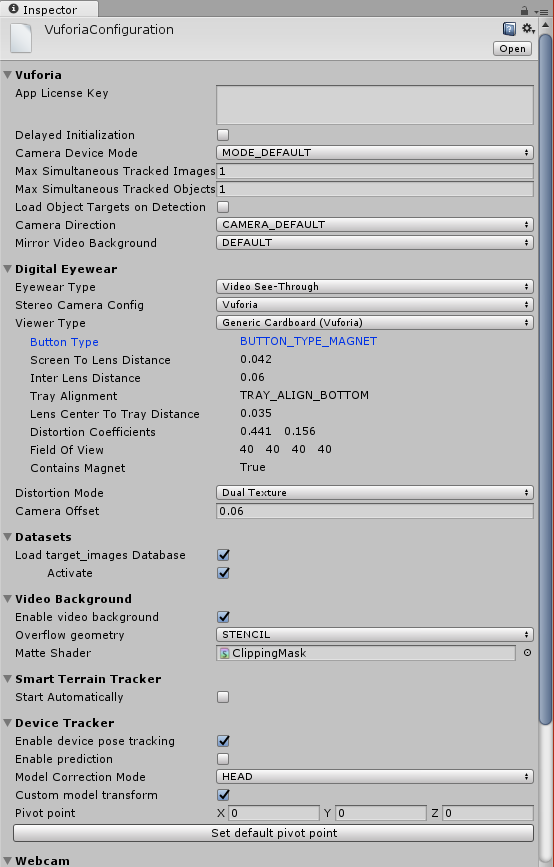
\includegraphics[width=0.5\textwidth]{img/inspector}
	\caption{Inspector Vuforia configuration}
	\label{fig:inspector}
\end{figure}

To combine it with the BullsEye framework, add the ServiceProvider script to the ARCamera object. 
If you downloaded an image target, search for the ImageTarget asset and drag it to the scene. Click on the ImageTarget object in the hierarchy and select the wished target image in the inspector under Image Target. Vuforia is now configured to look for the specified marker. You can add an gameobject to the scene and add it as a child of the ImageTarget object, like shown in \ref{fig:hierarchy_vuforia}. If Vuforia detects the marker the gameobject will be shown in the scene above the marker. 
\begin{figure}[htb]
	\centering
		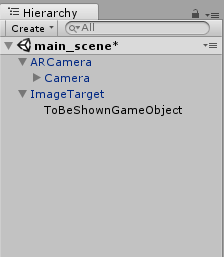
\includegraphics[width=0.5\textwidth]{img/vuforia_hierarchy}
	\caption{Hierarchy of GameObjects in the Unity Editor}
	\label{fig:hierarchy_vuforia}
\end{figure}



\end{document}